\newpage
\subsection{Учет готовой продукции}
\label{bp:readygoods}

Готовая подукция после линии упаковки на транспортной линии Para автоматически выходит на склад, где ее забирает водитель погрузчика.

Приемка выполняется водителями погрузчиков в течение дня через сканер ТСД “Перемещение ГП” (рис. \ref{pic:d_TSD_1}).
Водитель сканирует каждый паллет сканером ТСД. 
Кладовщик проверяет отчет по готовой продукции в системе 1С:УПП (форма \ref{pic:d31}).

По некоторым клиентами принимают только полные поддоны. Водитель погрузчика не принимает такие поддоны с производства. Списка таких клиентов нет, водители помнят по памяти. Такие поддоны водитель погрузчика снимает с линии упаковки и везет в цех.

В системе 1С:УПП ГП принимается документом “Перемещение товаров” с производства на склад ГП.
Кладовщик вручную проверяет данные в системе 1С:УПП по данным поступления.



% 30,
% 73) 
Кладовщик передает сдаточные акты в бухгалтерию.

Бухгалтерия дублирует вручную документы по готовой продукции в системе 1С:Бухгалерия.

\textbf{Возврат ГП}

Возврат готовой продукции выполняет только бухгалтерия через систему 1С:УПП. Бухгалтерия дублирует вручную документы по возврату в системе 1С:Бухгалерия.



\begin{figure}
\begin{center}
  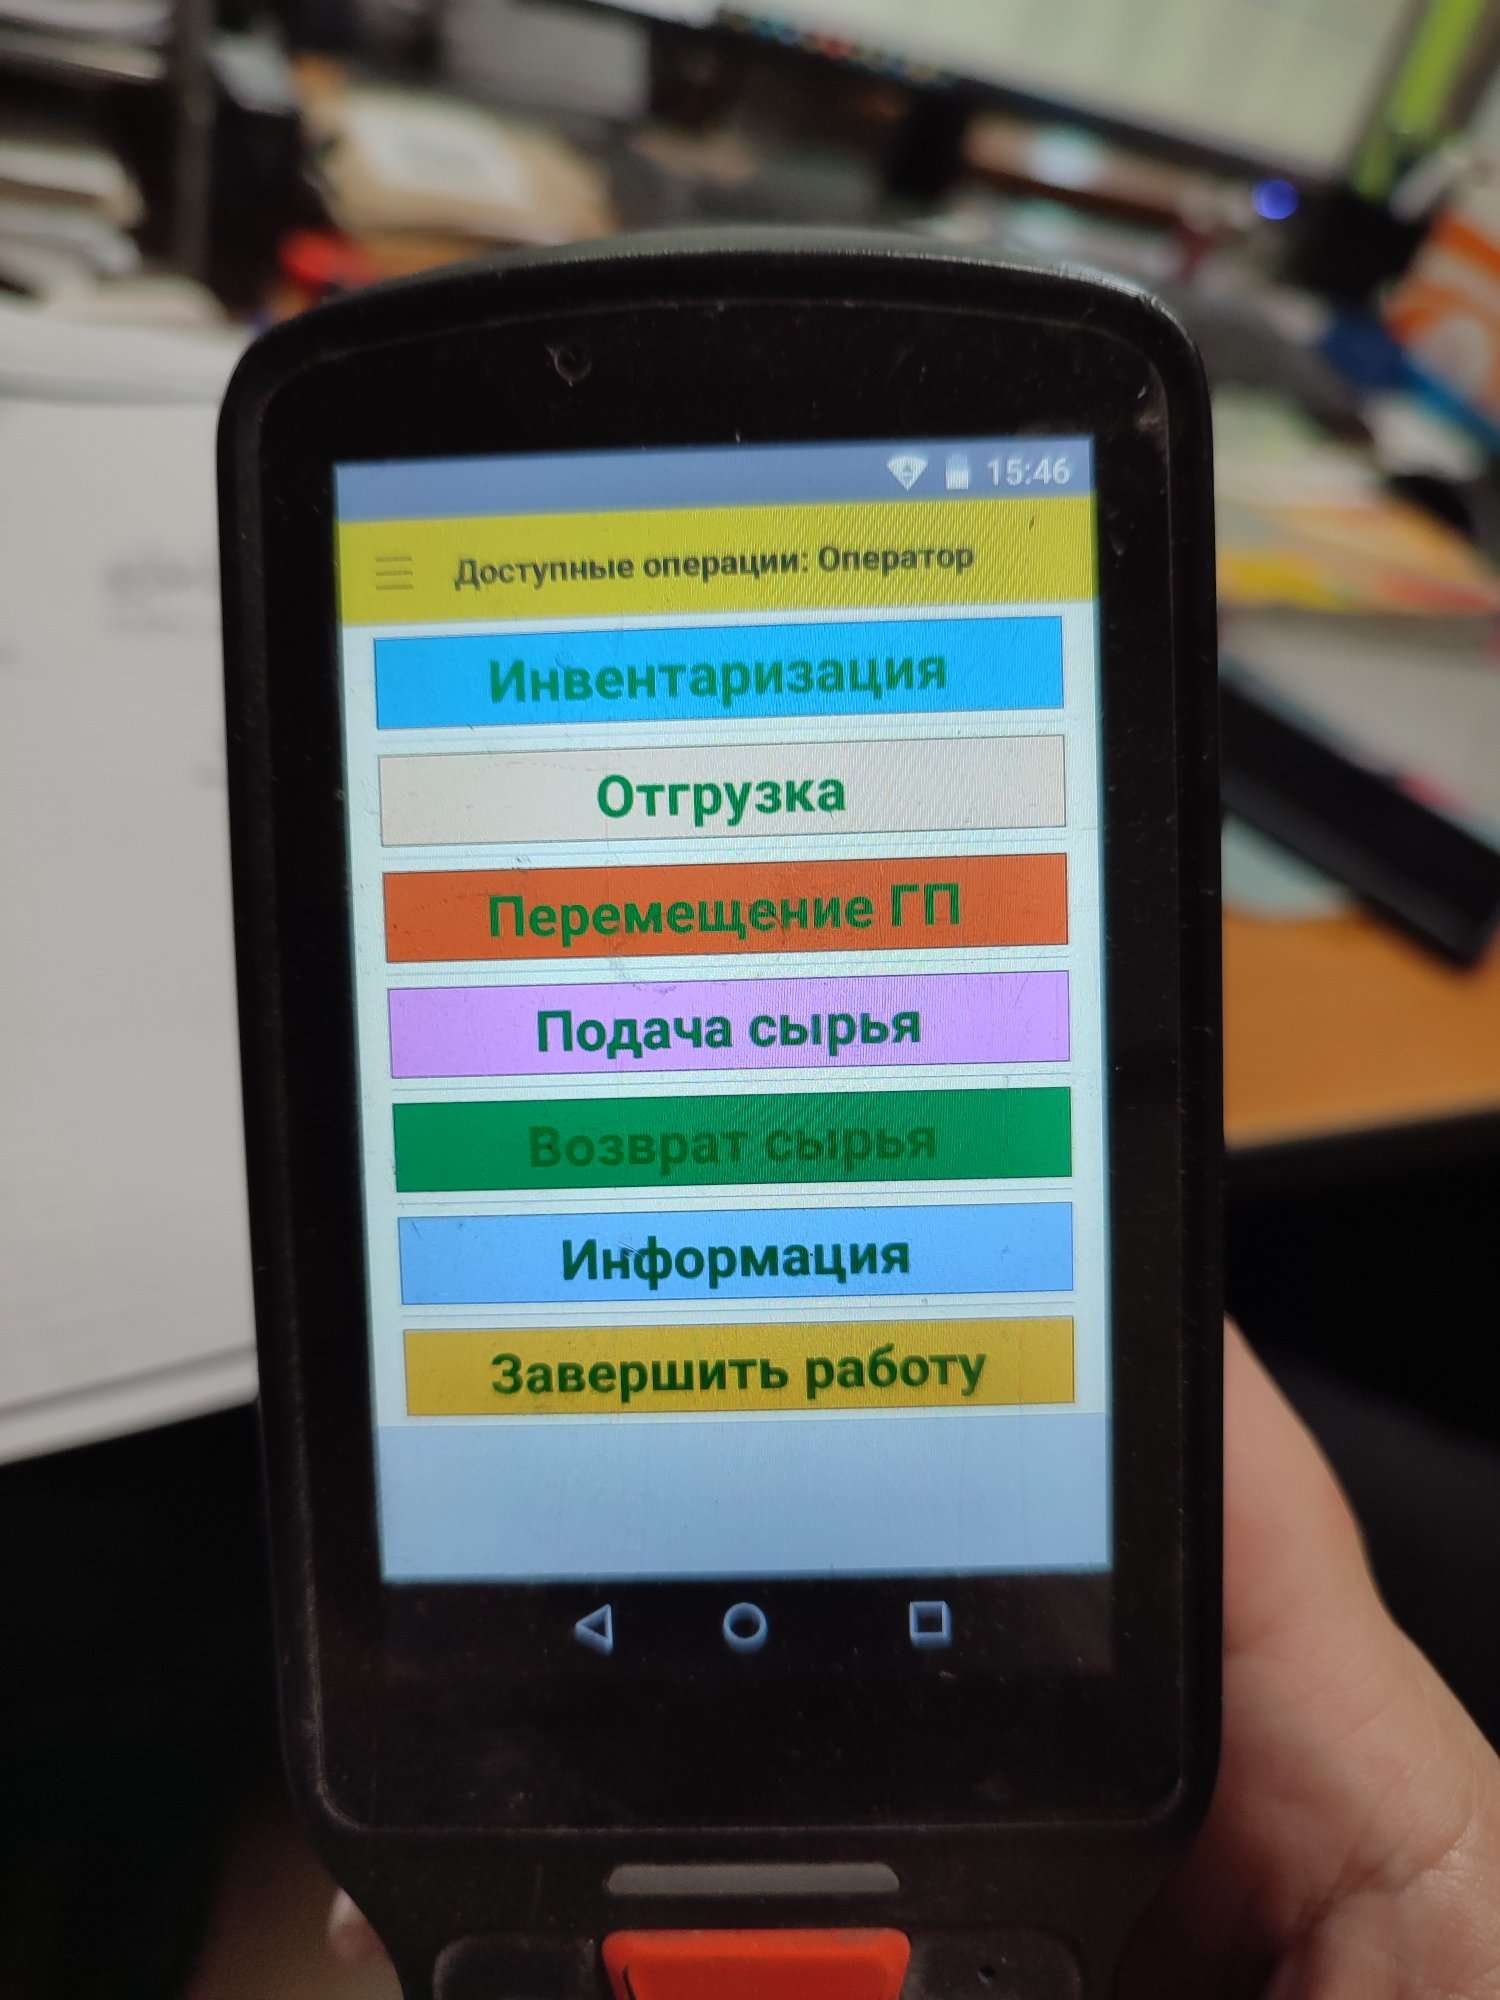
\includegraphics[height=0.94\textheight, width=\textwidth, keepaspectratio]{Pics/d_TSD_1.JPEG}
\end{center}
  \caption{Форма меню на ТСД}
  \label{pic:d_TSD_1}
\end{figure}


\begin{figure}
\begin{center}
  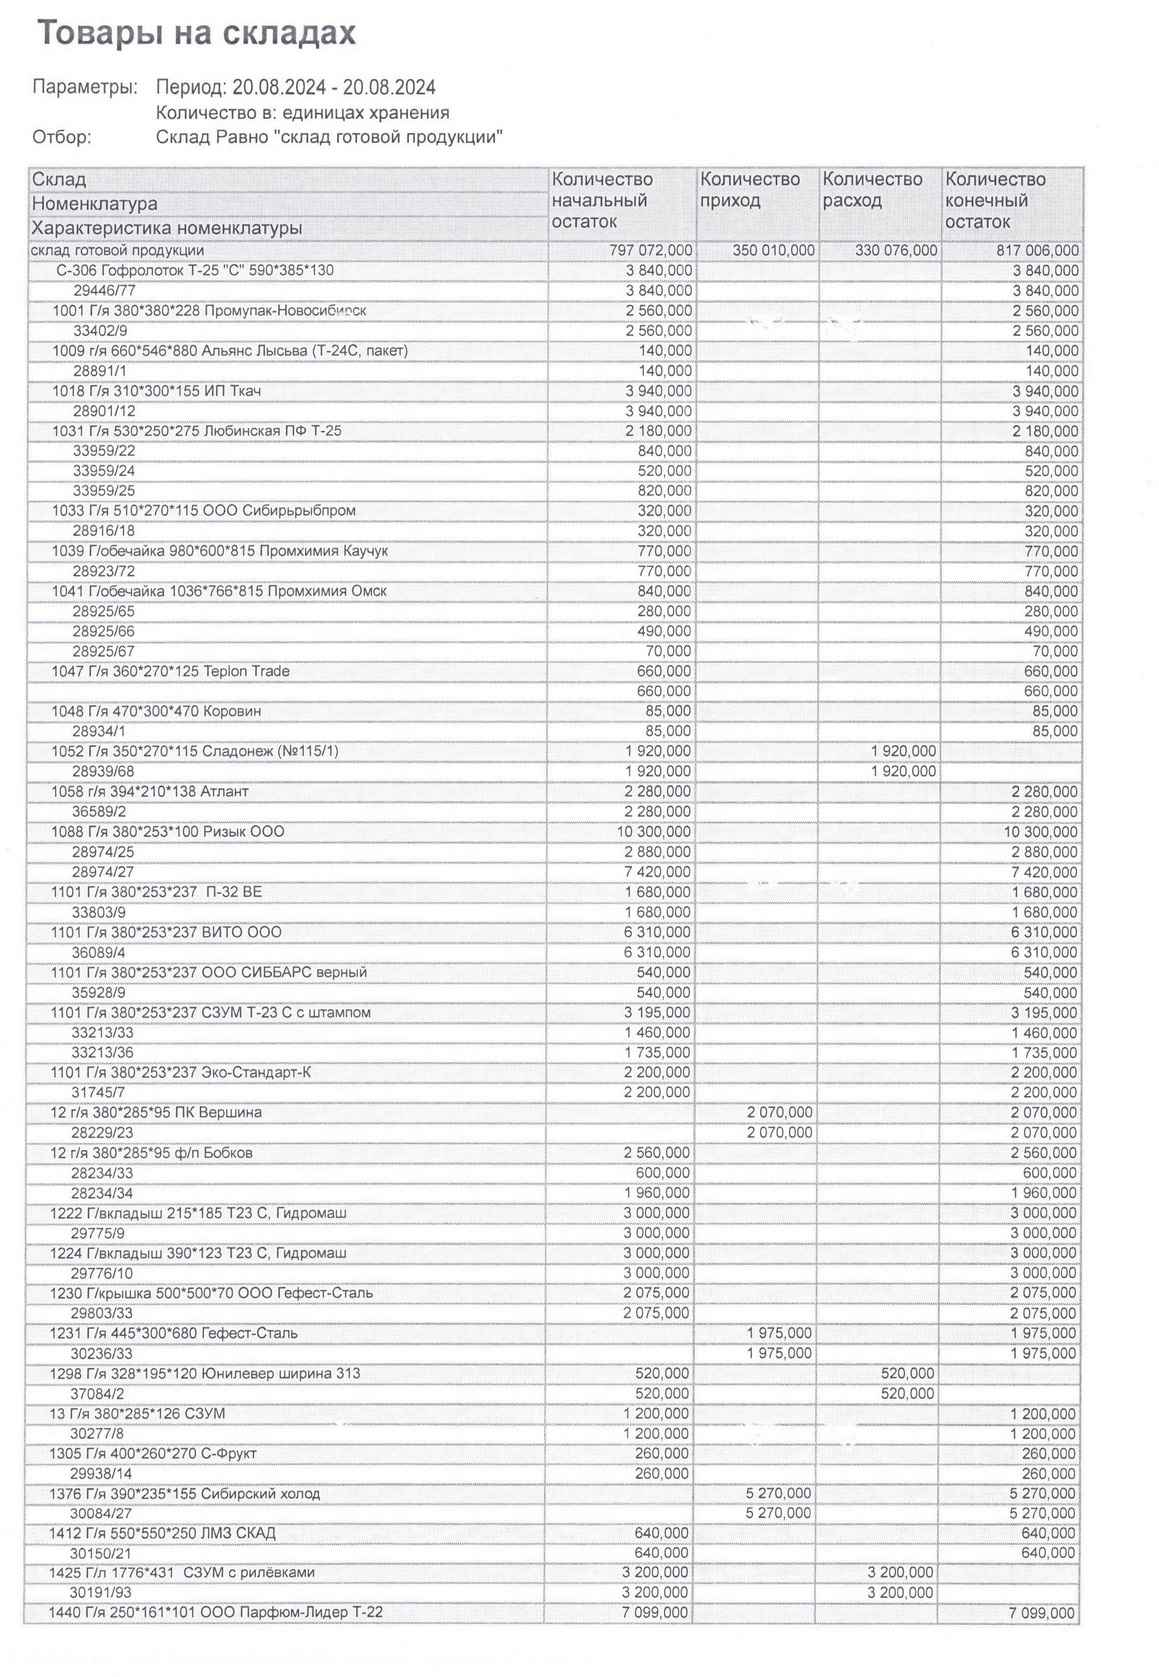
\includegraphics[height=0.94\textheight, width=\textwidth, keepaspectratio]{Pics/d31.jpg}
\end{center}
  \caption{Отчет по готовой продукции в системе 1С:УПП}
  \label{pic:d31}
\end{figure}




